\documentclass{article}
\usepackage{graphicx}
\usepackage{subfig}
\newcommand\mytab{\tab \hspace{+1cm}}
\usepackage{fancyhdr}
\usepackage{geometry}
\usepackage[most]{tcolorbox}
 \geometry{
 a4paper,
 total={170mm,257mm},
 left=20mm,
 top=20mm,
 }
\usepackage[utf8]{inputenc}
\linespread{1.15}
\usepackage{tikz,lipsum,lmodern}
\usepackage{hyperref}
\newtcolorbox{mybox}{
enhanced,
boxrule=0pt,frame hidden,
borderline west={4pt}{0pt}{green!75!black},
colback=green!10!white,
sharp corners
}
\newtcolorbox{mybox2}{
enhanced,
boxrule=0pt,frame hidden,
borderline west={4pt}{0pt}{blue!75!black},
colback=blue!10!white,
sharp corners
}
\usepackage{amsmath,amsfonts,amsthm,bm} % Math packages
\usepackage[most]{tcolorbox}
\usepackage{amssymb}
\hypersetup{
    colorlinks=true,
    linkcolor=blue,
    filecolor=magenta,      
    urlcolor=cyan,
    pdftitle={Overleaf Example},
    pdfpagemode=FullScreen,
    }
\usepackage{mathtools}
\usepackage{amsmath}

\usepackage{natbib}
\usepackage{wrapfig}
\usepackage{url}
\usepackage{pax}
\usepackage{pdfpages}
\usepackage{graphicx}
\usepackage{tikz}
\usepackage{blindtext}
\title{MA2001 Linear Algebra I AY1819 Sem 1 Final (Solutions)}
\author{Solution by Thang Pang Ern}

\begin{document}

\maketitle
\subsubsection*{Question 1}
\textbf{(a)} Consider the following matrix \[\mathbf{C}=\begin{pmatrix}1&2&-1&0\\2&5&-3&2\\2&4&-2&0\\3&8&-5&4\end{pmatrix}.\]
\textbf{(i)} Find a basis for the row space of $\mathbf{C}$.
\newline\newline\textit{Solution:} \[\operatorname{rref}(\mathbf{C})=\begin{pmatrix}1&0&1&-4\\0&1&-1&2\\0&0&0&0\\0&0&0&0\end{pmatrix}\]
Thus, a basis for the row space of $C$ is $\left\{(1,0,1,-4),(0,1,-1,2)\right\}$. An alternative solution would be using the original rows, which are $\left\{(1,2,-1,0),(2,5,-3,2)\right\}$. \qed 
\newline\newline\textbf{(ii)} Find a basis for the nullspace of $\mathbf{C}$. What is the rank and nullity of $\mathbf{C}$?
\newline
\newline\textit{Solution:} Consider \[\begin{pmatrix}1&0&1&-4\\0&1&-1&2\\0&0&0&0\\0&0&0&0\end{pmatrix}\begin{pmatrix}x_1\\x_2\\x_3\\x_4\end{pmatrix}=\begin{pmatrix}0\\0\\0\\0\end{pmatrix}.\] This is equivalent to solving \begin{align*}
    x_1+x_3-4x_4&=0\\
    x_2-x_3+2x_4&=0
\end{align*}
The solution to this system of equations is \[\begin{pmatrix}x_1\\x_2\\x_3\\x_4\end{pmatrix}=x_3\begin{pmatrix}-1\\1\\1\\0\end{pmatrix}+x_4\begin{pmatrix}4\\-2\\0\\1\end{pmatrix},\text{ where }x_3,x_4\in\mathbb{R}.\] Hence, a basis for the nullspace of $\mathbf{C}$ is \[\left\{\begin{pmatrix}-1\\1\\1\\0\end{pmatrix},\begin{pmatrix}4\\-2\\0\\1\end{pmatrix}\right\}.\] So $\operatorname{nullity}(\mathbf{C})=2$ and thus, by the Rank-Nullity Theorem, $\operatorname{rank}(\mathbf{C})=2$. \qed
\newline
\newline\textbf{(iii)} Is the last row of $\mathbf{C}$ a linear combination of the other rows of $\mathbf{C}$? If it is, find such a linear combination.
If it is not, explain why.
\newline
\newline\textit{Solution:} Yes, the last row of $\mathbf{C}$ is a linear combination of the other rows since $\operatorname{rank}(\mathbf{C})=2 < 4$. Consider \[\begin{pmatrix}3\\8\\-5\\4\end{pmatrix}=\alpha\begin{pmatrix}1\\2\\-1\\0\end{pmatrix}+\beta\begin{pmatrix}2\\5\\-3\\2\end{pmatrix}+\gamma\begin{pmatrix}2\\4\\-2\\0\end{pmatrix}.\]
Solving yields $\alpha=-1-2\gamma$, $\beta=2$ for $\gamma\in\mathbb{R}$. Thus, we can set $\gamma=0$, resulting in $\alpha=-1$. Therefore, \[\begin{pmatrix}3\\8\\-5\\4\end{pmatrix}=-\begin{pmatrix}1\\2\\-1\\0\end{pmatrix}+2\begin{pmatrix}2\\5\\-3\\2\end{pmatrix}.\] \qed
\newline
\newline\textbf{(b)} Suppose $\mathbf{D}$ is a matrix with $k$ columns such that the linear system $\mathbf{Dx}=\mathbf{r}$ is consistent for all vectors $\mathbf{r}\in\mathbb{R}^n$. For each of the statements below, determine if the statement is true. Justify your answer.
\newline
\newline\textbf{(i)} $\mathbf{D}$ has $n$ rows.
\newline\textit{Solution:} True since $\mathbf{r}$ is of size $n\times 1$. \qed 
\newline
\newline\textbf{(ii)} $k$ is at least $n$
\newline\textit{Solution:} True as this can be regarded as a system of $n$ equations with $k$ unknowns. \qed 
\newline
\newline\textbf{(iii)} $\mathbf{D}$ is of full rank.
\newline\textit{Solution:} Note that $\operatorname{rank}(\mathbf{D})\le \operatorname{min}(n,k)$ because $\mathbf{D}$ cannot have more pivots than rows or columns. From \textbf{(ii)}, as $k \ge n$, then $\operatorname{min}(n,k)=n$ so $\operatorname{rank}(\mathbf{D})\le n$. Since the linear system $\mathbf{Dx}=\mathbf{r}$ is consistent, then in the augmented matrix $\left(\mathbf{D}|\mathbf{r}\right)$, there does not exist a pivot in the rightmost column, and so, the row-echelon form of $\mathbf{D}$ has no zero rows. Hence, $\operatorname{rank}(\mathbf{D})=n$. \qed 
\subsubsection*{Question 2}
\textbf{(a)} $\mathbf{A}$ is a square matrix of order 10 with entries $a_{ij}$ such that $\operatorname{det}(\mathbf{A})=2$. Let $\mathbf{B}$ be another square matrix of order 10 such that \[{{b}_{ij}}=\left\{ \begin{matrix}
   -\frac{1}{2}{{a}_{ij}} & \text{if }i\text{ is odd;}  \\
   2{{a}_{ij}} & \text{if }i\text{ is even}\text{.}  \\
\end{matrix} \right.\]
Find $\operatorname{det}(\mathbf{B})$.
\newline
\newline\textit{Solution:} \[\operatorname{det}(\mathbf{B})=\left(-\frac{1}{2} \cdot 2\right)^5\det(\mathbf{A})=-\det(\mathbf{A})\] \qed 
\newline
\newline
\textbf{(b)} Let \[\mathbf{B}=\begin{pmatrix}1&2&4\\-1&10&5\\1&-2&3\end{pmatrix}.\]
Perform three elementary row operations to reduce $\mathbf{B}$ to a row-echelon form. Hence find three elementary matrices $\mathbf{E}_1,\mathbf{E}_2,\mathbf{E}_3$ such that $\mathbf{B}^\text{T}\mathbf{E}_1\mathbf{E}_2\mathbf{E}_3$ is a lower triangular matrix. Write down the elementary row operations that $\mathbf{E}_1,\mathbf{E}_2,\mathbf{E}_3$ represent respectively.
\newline
\newline\textit{Solution:} \[\mathbf{B}=\left( \begin{matrix}
   1 & 2 & 4  \\
   -1 & 10 & 5  \\
   1 & -2 & 3  \\
\end{matrix} \right)\xrightarrow{{{R}_{1}}+{{R}_{2}}\to {{R}_{2}}}\left( \begin{matrix}
   1 & 2 & 4  \\
   0 & 12 & 9  \\
   1 & -2 & 3  \\
\end{matrix} \right)\xrightarrow{-{{R}_{1}}+{{R}_{3}}\to {{R}_{3}}}\left( \begin{matrix}
   1 & 2 & 4  \\
   0 & 12 & 9  \\
   0 & -4 & -1  \\
\end{matrix} \right)\xrightarrow{\frac{1}{3}{{R}_{2}}+{{R}_{3}}\to {{R}_{3}}}\left( \begin{matrix}
   1 & 2 & 4  \\
   0 & 12 & 9  \\
   0 & 0 & 2  \\
\end{matrix} \right)\]
Thus, \[{{\mathbf{F}}_{1}}=\left( \begin{matrix}
   1 & 0 & 0  \\
   1 & 1 & 0  \\
   0 & 0 & 1  \\
\end{matrix} \right),\text{ }{{\mathbf{F}}_{2}}=\left( \begin{matrix}
   1 & 0 & 0  \\
   0 & 1 & 0  \\
   -1 & 0 & 1  \\
\end{matrix} \right)\text{ and }{{\mathbf{F}}_{3}}=\left( \begin{matrix}
   1 & 0 & 0  \\
   0 & 1 & 0  \\
   0 & \frac{1}{3} & 1  \\
\end{matrix} \right).\]
Since $\mathbf{F}_3\mathbf{F}_2\mathbf{F}_1\mathbf{B}$ is upper triangular, taking transpose, $\mathbf{B}^\text{T}\mathbf{F}_1^\text{T}\mathbf{F}_2^\text{T}\mathbf{F}_3^\text{T}$ must be lower triangular. Thus, $\mathbf{E}_i=\mathbf{F}_i^\text{T}$ for $i=1,2,3$. That is, \[\mathbf{E}_1=\begin{pmatrix}1&1&0\\0&1&0\\0&0&1
\end{pmatrix}, \text{ }\mathbf{E}_2=\begin{pmatrix}1&0&-1\\0&1&0\\0&0&1
\end{pmatrix}\text{ and }\mathbf{E}_3=\begin{pmatrix}1&0&0\\0&1&\frac{1}{3}\\0&0&1
\end{pmatrix}.\]
As for what each of the $\mathbf{E}_i$'s represents,
\begin{itemize}
    \item $\mathbf{E}_1$ denotes adding row 2 to row 1
    \item $\mathbf{E}_2$ denotes adding negative of row 3 to row 1
    \item $\mathbf{E}_3$ denotes adding $1/3$ of row 3 to row 2
\end{itemize} \qed 
\newline
\newline\textbf{\textcolor{purple}{Remark:}} This is similar to the notion of $LU$ decomposition, which says that a matrix $\mathbf{A}$ can be \textit{decomposed} into a lower triangular matrix $\mathbf{L}$ and an upper triangular matrix $\mathbf{U}$. The study of this technique is essential in the field of Numerical Analysis.
\newline
\newline\textbf{(c)} Let $\mathbf{X}$ and $\mathbf{Y}$ be square matrices of the same order. Prove the following statements.
\newline
\newline\textbf{(i)} $\mathbf{X}^\text{T}\mathbf{X}=\mathbf{0}$ if and only if $\mathbf{X}=\mathbf{0}$. (Hint: Consider the diagonal entries of $\mathbf{X}^\text{T}\mathbf{X}$)
\newline
\newline\textit{Solution:} If $\mathbf{X}=\mathbf{0}$, then $\mathbf{X}^\text{T}=\mathbf{0}$, so $\mathbf{X}^\text{T}\mathbf{X}=\mathbf{0}$.
\newline
\newline Now, we prove that if $\mathbf{X}^\text{T}\mathbf{X}=\mathbf{0}$, then $\mathbf{X}=\mathbf{0}$. Suppose $\mathbf{X}$ is of order $n$. Note that the $(i,j)$-entry of $\mathbf{X}$ is denoted by $x_{ij}$, where $1 \le i,j \le n$. Also, the $(i,j)$-entry of $\mathbf{X}^\text{T}$ is denoted by $x_{ji}$. By matrix multiplication, the $(j,j)$-entry of $\mathbf{X}^\text{T}\mathbf{X}$ is \[\sum_{i=1}^{n}x_{ij}^2=0.\] That is, each diagonal entry of $\mathbf{X}^\text{T}\mathbf{X}$ is represented by the above sum. We have $x_{ij}^2=0$ for all $1 \le i,j \le n$, and therefore, $x_{ij}=0$. The result follows. \qed 
\newline
\newline\textbf{(ii)} $\mathbf{XY}=\mathbf{0}$ if and only if $\mathbf{X}^\text{T}\mathbf{XY}=\mathbf{0}$. (Hint: Use \textbf{(i)})
\newline
\newline\textit{Solution:} $\mathbf{XY}=\mathbf{0}$ implies $\mathbf{X}^\text{T}\mathbf{XY}=\mathbf{0}$ is trivial.
\newline
\newline Now, suppose $\mathbf{X}^\text{T}\mathbf{XY}=\mathbf{0}$. Then, \begin{align*}
    \mathbf{Y}^\text{T}\mathbf{X}^\text{T}\mathbf{XY}&=\mathbf{Y}^\text{T}\mathbf{0}\\
    (\mathbf{X}\mathbf{Y})^\text{T}(\mathbf{XY})&=\mathbf{0}
\end{align*}
The result follows. \qed 
\newpage
\subsubsection*{Question 3}
\textbf{(a)} Let $V=\left\{(a-b,a-2b,a+b,a+3b)|a,b\in\mathbb{R}\right\}$
\newline
\newline\textbf{(i)} Show that $V$ is a subspace of $\mathbb{R}^4$.
\newline
\newline\textit{Solution:} Setting $a=b=0$, the zero vector is contained in $V$, so $V$ is non-empty.
\newline
\newline Let $\mathbf{v}_1=(a_1-b_1,a_1-2b_1,a_1+b_1,a_1+3b_1)$ and $\mathbf{v}_2=(a_2-b_2,a_2-2b_2,a_2+b_2,a_2+3b_2)$ be in $V$. For $\alpha\in\mathbb{R}$, 	\begin{align*}
 & \alpha {{\mathbf{v}}_{1}}+{{\mathbf{v}}_{2}} \\
 &=\alpha \left( {{a}_{1}}-{{b}_{1}},{{a}_{1}}-2{{b}_{1}},{{a}_{1}}+{{b}_{1}},{{a}_{1}}+3{{b}_{1}} \right)+\left( {{a}_{2}}-{{b}_{2}},{{a}_{2}}-2{{b}_{2}},{{a}_{2}}+{{b}_{2}},{{a}_{2}}+3{{b}_{2}} \right)\\
 &=\left( \alpha \left( {{a}_{1}}-{{b}_{1}} \right),\alpha \left( {{a}_{1}}-2{{b}_{1}} \right),\alpha \left( {{a}_{1}}+{{b}_{1}} \right),\alpha \left( {{a}_{1}}+3{{b}_{1}} \right) \right)+\left( {{a}_{2}}-{{b}_{2}},{{a}_{2}}-2{{b}_{2}},{{a}_{2}}+{{b}_{2}},{{a}_{2}}+3{{b}_{2}} \right)\\
 &=\left( \alpha \left( {{a}_{1}}-{{b}_{1}} \right)+{{a}_{2}}-{{b}_{2}},\alpha \left( {{a}_{1}}-2{{b}_{1}} \right)+{{a}_{2}}-2{{b}_{2}},\alpha \left( {{a}_{1}}+{{b}_{1}} \right)+{{a}_{2}}+{{b}_{2}},\alpha \left( {{a}_{1}}+3{{b}_{1}} \right)+{{a}_{2}}+3{{b}_{2}} \right)\\
 &=(\alpha a_1+a_2-\alpha b_1-b_2,\alpha a_1+a_2-2\alpha b_1-2b_2,\alpha a_1+a_2+\alpha b_1+b_2,\alpha a_1+a_2+3\alpha b_1+3b_2) 
\end{align*}
which shows that $V$ is closed under addition and scalar multiplication.\qed
\newline
\newline\textbf{(ii)} Find a basis for $V$. What is the dimension of $V$?
\newline
\newline\textit{Solution:} Note that each vector in $V$ can be written as $a(1,1,1,1)+b(-1,-2,1,3)$ so a basis for $V$ is $\left\{(1,1,1,1),(-1,-2,1,3)\right\}$. Also, $\operatorname{dim}(V)=2$. \qed 
\newline
\newline\textbf{(iii)} Let $W$ be the solution space of the following homogeneous linear system:
\begin{align*}
    x_1-x_2+x_3+x_4&=0\\
    x_2-x_3+6x_4&=0\\
    x_3+3x_4&=0
\end{align*}
Find a basis for $W$ and hence show that $W \subseteq V$.
\newline
\newline\textit{Solution:} By backward substitution, $x_1=-7x_4$, $x_2=-9x_4$ and $x_3=-3x_4$. Hence, a basis for $W$ is $\left\{(-7,-9,-3,1)\right\}$. As $(-7,-9,-3,1)=-5(1,1,1,1)+2(-1,-2,1,3)$, then $W\subseteq V$. \qed 
\newline\newline\textbf{(b)} Let $E=\left\{(1,0),(0,1)\right\}$ and $S=\left\{(1,1),(1,-1)\right\}$.
\newline\textbf{(i)} $E$ is the standard basis for $\mathbb{R}^2$. Is $S$ also a basis for $\mathbb{R}^2$? Justify your answer.
\newline
\newline\textit{Solution:} $S$ spans $\mathbb{R}^2$. This is evident as \[\left( \left. \begin{matrix}
   1 & 1  \\
   1 & -1  \\
\end{matrix} \right|\begin{matrix}
   x  \\
   y  \\
\end{matrix} \right)\xrightarrow{-{{R}_{1}}+{{R}_{2}}\to {{R}_{2}}}\left( \left. \begin{matrix}
   1 & 1  \\
   0 & -2  \\
\end{matrix} \right|\begin{matrix}
   x  \\
   y-x  \\
\end{matrix} \right)\] which shows that the above system is consistent for any $x,y\in\mathbb{R}$. Consider $\alpha(1,1)+\beta(1,-1)=(0,0)$. Then, $\alpha+\beta=0$ and $\alpha-\beta=0$. Thus, $\alpha=\beta=0$, implying that these vectors are linearly independent. Hence, $S$ is also a basis for $\mathbb{R}^2$. \qed 
\newpage
\textbf{(ii)} The triangle in the right figure is re-drawn exactly on the left figure as shown. Find the coordinates of the 3 points $a,b$ and $c$, with respect to the coordinates used in the left figure. The coordinates of $A,B$ and $C$ are given by $(1.2,2.2), (3.2,3.2)$ and $(2.2,4.8)$ respectively.
\begin{figure}[h!]
\centering
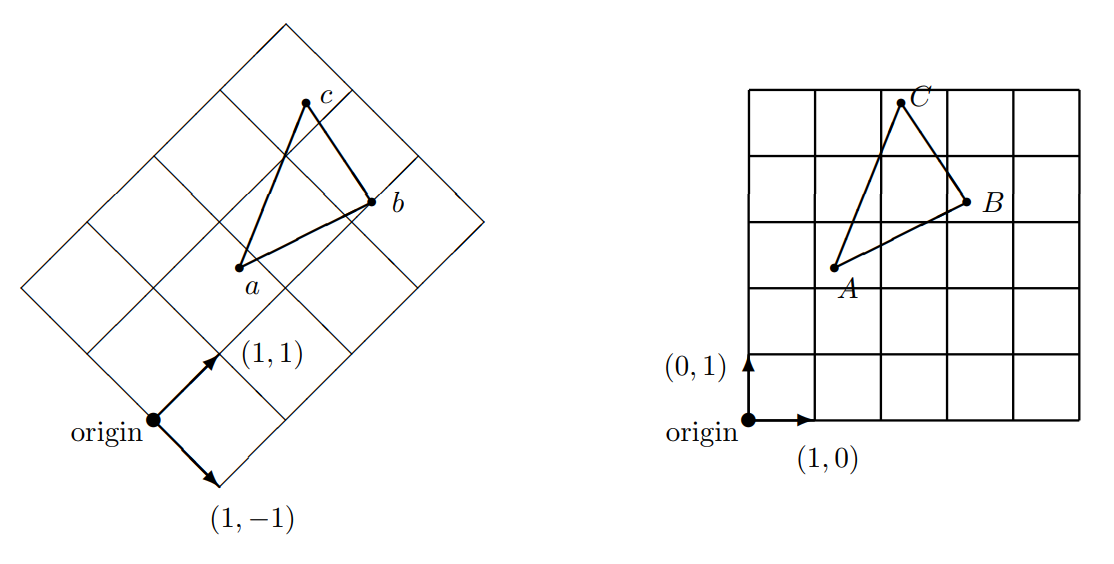
\includegraphics[width=0.75\textwidth]{Vector.png}
\end{figure}
\newblock
\newline\textit{Solution:} Bases for $S_1$ and $S_2$ are \[{{S}_{1}}=\left\{ \left( \begin{matrix}
  1 \\ 
  -1 \\ 
\end{matrix} \right),\left( \begin{matrix}
  1 \\ 
  1 \\ 
\end{matrix} \right) \right\}\text{ and }{{S}_{2}}=\left\{ \left( \begin{matrix}
  1 \\ 
  0 \\ 
\end{matrix} \right),\left( \begin{matrix}
  0 \\ 
  1 \\ 
\end{matrix} \right) \right\}.\] We see that \[{{\left[ \left( \begin{matrix}
  0 \\ 
  1 \\ 
\end{matrix} \right) \right]}_{{{S}_{2}}}}=\left( \begin{matrix}
  1 \\ 
  0 \\ 
\end{matrix} \right)=\frac{1}{2}\left[ \left( \begin{matrix}
  1 \\ 
  1 \\ 
\end{matrix} \right)+\left( \begin{matrix}
  1 \\ 
  -1 \\ 
\end{matrix} \right) \right]={{\left[ \left( \begin{matrix}
  \frac{1}{2} \\ 
  \frac{1}{2} \\ 
\end{matrix} \right) \right]}_{{{S}_{1}}}}\]
and \[{{\left[ \left( \begin{matrix}
  1 \\ 
  0 \\ 
\end{matrix} \right) \right]}_{{{S}_{2}}}}=\left( \begin{matrix}
  0 \\ 
  1 \\ 
\end{matrix} \right)=\frac{1}{2}\left[ \left( \begin{matrix}
  1 \\ 
  1 \\ 
\end{matrix} \right)-\left( \begin{matrix}
  1 \\ 
  -1 \\ 
\end{matrix} \right) \right]={{\left[ \left( \begin{matrix}
  \frac{1}{2} \\ 
  -\frac{1}{2} \\ 
\end{matrix} \right) \right]}_{{{S}_{1}}}}\]
so the transition matrix is \[\left( \begin{matrix}
   \frac{1}{2} & \frac{1}{2}  \\
   \frac{1}{2} & -\frac{1}{2}  \\
\end{matrix} \right).\]
 The position vector representing the point $a$ can be found by \[\begin{pmatrix}
   \frac{1}{2} & \frac{1}{2}  \\
   \frac{1}{2} & -\frac{1}{2} 
\end{pmatrix}\begin{pmatrix}1.2\\2.2\end{pmatrix}.\] The same can be said for $b$ and $c$.
\newline
\newline Hence, $a=(-0.5,1.7)$, $b=(0,3.2)$ and $c=(-1.3,3.5)$. \qed 
\subsubsection*{Question 4}
Let $V=\operatorname{span}\left\{\mathbf{u}_1,\mathbf{u}_2,\mathbf{u}_3\right\}$, where \[\mathbf{u}_1=\begin{pmatrix}1\\1\\1\\1\end{pmatrix},\mathbf{u}_2=\begin{pmatrix}0\\1\\1\\0\end{pmatrix}\text{ and }\mathbf{u}_3=\begin{pmatrix}0\\1\\0\\2\end{pmatrix}.\]
\textbf{(i)} Find a vector $\mathbf{u}$ such that $\left\| \mathbf{u} \right\|=3\sqrt{10}$ and $\mathbf{u}$ is orthogonal to $\mathbf{u}_1,\mathbf{u}_2$ and $\mathbf{u}_3$.
\newline
\newline\textit{Solution:} Let \[\mathbf{u}=\begin{pmatrix}a\\b\\c\\d\end{pmatrix}.\] By considering orthogonality, we can form three equations: \begin{align*}
    a+b+c+d&=0\\
    b+c&=0\\
    b+2d&=0
\end{align*}
Using the norm of $\mathbf{u}$, we have \[a^2+b^2+c^2+d^2=90.\] Solving the first three equations by backward substitution yields $a=-d$, $b=-2d$ and $c=2d$. Substituting these into the equation representing the norm of $\mathbf{u}$, \[d^2+4d^2+4d^2+d^2=90.\] Thus, $d=3$ ($d=-3$ also works as there is no restriction). So, $a=-3$, $b=-6$ and $d=6$. A vector $\mathbf{u}$ is \[\begin{pmatrix} -3\\-6\\6\\3\end{pmatrix}.\] \qed
\newline
\newline\textbf{(ii)} Use the Gram-Schmidt Process to transform $\left\{\mathbf{u}_1,\mathbf{u}_2,\mathbf{u}_3\right\}$ into an orthonormal basis for $V$.
\newline
\newline\textit{Solution:} Note that $\left\| {{\mathbf{u}}_{1}} \right\|=4$ so \[\mathbf{v}_1=\left( \begin{matrix}
   \frac{1}{2}  \\
   \frac{1}{2}  \\
   \frac{1}{2}  \\
   \frac{1}{2}  \\
\end{matrix} \right).\] \ Using the Gram-Schmidt Process, \[{{\mathbf{v}}_{2}}=\left( \begin{matrix}
  0 \\ 
  1 \\ 
  1 \\ 
  0 \\ 
\end{matrix} \right)-\left( \left( \begin{matrix}
  0 \\ 
  1 \\ 
  1 \\ 
  0 \\ 
\end{matrix} \right)\cdot \left( \begin{matrix}
   \frac{1}{2}  \\
   \frac{1}{2}  \\
   \frac{1}{2}  \\
   \frac{1}{2}  \\
\end{matrix} \right) \right)\left( \begin{matrix}
   \frac{1}{2}  \\
   \frac{1}{2}  \\
   \frac{1}{2}  \\
   \frac{1}{2}  \\
\end{matrix} \right)=\left( \begin{matrix}
   -\frac{1}{2}  \\
   \frac{1}{2}  \\
   \frac{1}{2}  \\
   -\frac{1}{2}  \\
\end{matrix} \right).\]
Using the Gram-Schmidt Process again, \[{{\mathbf{v}}_{3}}=\left( \begin{matrix}
  0 \\ 
  1 \\ 
  0 \\ 
  2 \\ 
\end{matrix} \right)-\left( \left( \begin{matrix}
  0 \\ 
  1 \\ 
  0 \\ 
  2 \\ 
\end{matrix} \right)\cdot \left( \begin{matrix}
   \frac{1}{2}  \\
   \frac{1}{2}  \\
   \frac{1}{2}  \\
   \frac{1}{2}  \\
\end{matrix} \right) \right)\left( \begin{matrix}
   \frac{1}{2}  \\
   \frac{1}{2}  \\
   \frac{1}{2}  \\
   \frac{1}{2}  \\
\end{matrix} \right)-\left( \left( \begin{matrix}
  0 \\ 
  1 \\ 
  0 \\ 
  2 \\ 
\end{matrix} \right)\cdot \left( \begin{matrix}
   -\frac{1}{2}  \\
   \frac{1}{2}  \\
   \frac{1}{2}  \\
   -\frac{1}{2}  \\
\end{matrix} \right) \right)\left( \begin{matrix}
   -\frac{1}{2}  \\
   \frac{1}{2}  \\
   \frac{1}{2}  \\
   -\frac{1}{2}  \\
\end{matrix} \right)=\left( \begin{matrix}
   -\sqrt{\frac{2}{5}}  \\
   \frac{1}{\sqrt{10}}  \\
   -\frac{1}{\sqrt{10}}  \\
   \sqrt{\frac{2}{5}}  \\
\end{matrix} \right)\]
so we conclude that
\[{{\mathbf{v}}_{1}}=\left( \begin{matrix}
   \frac{1}{2}  \\
   \frac{1}{2}  \\
   \frac{1}{2}  \\
   \frac{1}{2}  \\
\end{matrix} \right),{{\mathbf{v}}_{2}}=\left( \begin{matrix}
   -\frac{1}{2}  \\
   \frac{1}{2}  \\
   \frac{1}{2}  \\
   -\frac{1}{2}  \\
\end{matrix} \right)\text{ and }{{\mathbf{v}}_{3}}=\left( \begin{matrix}
   -\sqrt{\frac{2}{5}}  \\
   \frac{1}{\sqrt{10}}  \\
   -\frac{1}{\sqrt{10}}  \\
   \sqrt{\frac{2}{5}}  \\
\end{matrix} \right),\] where $\left\{\mathbf{v}_1,\mathbf{v}_2,\mathbf{v}_3\right\}$ is an orthonormal basis for $V$. \qed
\newline
\newline\textbf{(iii)} Find the projection of \[\mathbf{w}=\begin{pmatrix}-1\\1\\-1\\13\end{pmatrix}\] onto $V$.
\newline
\newline\textit{Solution:} The projection is \begin{align*}
  & \left( \left( \begin{matrix}
   -1  \\
   1  \\
   -1  \\
   13  \\
\end{matrix} \right)\cdot \left( \begin{matrix}
   \frac{1}{2}  \\
   \frac{1}{2}  \\
   \frac{1}{2}  \\
   \frac{1}{2}  \\
\end{matrix} \right) \right)\left( \begin{matrix}
   \frac{1}{2}  \\
   \frac{1}{2}  \\
   \frac{1}{2}  \\
   \frac{1}{2}  \\
\end{matrix} \right)+\left( \left( \begin{matrix}
   -1  \\
   1  \\
   -1  \\
   13  \\
\end{matrix} \right)\cdot \left( \begin{matrix}
   -\frac{1}{2}  \\
   \frac{1}{2}  \\
   \frac{1}{2}  \\
   -\frac{1}{2}  \\
\end{matrix} \right) \right)\left( \begin{matrix}
   -\frac{1}{2}  \\
   \frac{1}{2}  \\
   \frac{1}{2}  \\
   -\frac{1}{2}  \\
\end{matrix} \right)+\left( \left( \begin{matrix}
   -1  \\
   1  \\
   -1  \\
   13  \\
\end{matrix} \right)\cdot \left( \begin{matrix}
   -\sqrt{\frac{2}{5}}  \\
   \frac{1}{\sqrt{10}}  \\
   -\frac{1}{\sqrt{10}}  \\
   \sqrt{\frac{2}{5}}  \\
\end{matrix} \right) \right)\left( \begin{matrix}
   -\sqrt{\frac{2}{5}}  \\
   \frac{1}{\sqrt{10}}  \\
   -\frac{1}{\sqrt{10}}  \\
   \sqrt{\frac{2}{5}}  \\
\end{matrix} \right)\\&=6\left( \begin{matrix}
   \frac{1}{2}  \\
   \frac{1}{2}  \\
   \frac{1}{2}  \\
   \frac{1}{2}  \\
\end{matrix} \right)-6\left( \begin{matrix}
   -\frac{1}{2}  \\
   \frac{1}{2}  \\
   \frac{1}{2}  \\
   -\frac{1}{2}  \\
\end{matrix} \right)+\sqrt{90}\left( \begin{matrix}
   -\sqrt{\frac{2}{5}}  \\
   \frac{1}{\sqrt{10}}  \\
   -\frac{1}{\sqrt{10}}  \\
   \sqrt{\frac{2}{5}}  \\
\end{matrix} \right) \\ 
 & =\left( \begin{matrix}
   0\\3\\-3\\12
\end{matrix} \right)  
\end{align*}\qed
\newline
\newline\textbf{(iv)} Let $A=\begin{pmatrix}\mathbf{u}_1&\mathbf{u}_2&\mathbf{u}_3\end{pmatrix}$, where $\mathbf{u}_1,\mathbf{u}_2$ and $\mathbf{u}_3$ are the columns of $\mathbf{A}$. Find a least squares solution to the linear system $\mathbf{Ax}=\mathbf{w}$.
\newline
\newline\textit{Solution:} We have \[\mathbf{A}=\begin{pmatrix}1&0&0\\1&1&1\\1&1&0\\1&0&2\end{pmatrix}.\] Consider $\mathbf{A}^\text{T}\mathbf{Ax}=\mathbf{A}^\text{T}\mathbf{w}$, so \[\begin{pmatrix}4&2&3\\2&2&1\\3&1&5\end{pmatrix}\mathbf{x}=\begin{pmatrix}12\\0\\27\end{pmatrix},\] hence, a least squares solution is \[\mathbf{x}=\begin{pmatrix}0\\-3\\6\end{pmatrix}.\]\qed
\subsubsection*{Question 5}
\textbf{(a)} Let \[\mathbf{A}=\begin{pmatrix}2&0&0\\-1&1&3\\1&1&-1\end{pmatrix}.\] \textbf{(i)} Find all the eigenvalues of $\mathbf{A}$.
\newline
\newline \textit{Solution:} \[\det (\mathbf{A}-\lambda \mathbf{I})=\operatorname{det}\left(\left( \begin{matrix}
   2-\lambda  & 0 & 0  \\
   -1 & 1-\lambda  & 3  \\
   1 & 1 & -1-\lambda   \\
\end{matrix} \right)\right)\]
Setting the determinant to be zero,
\begin{align*}
    (2-\lambda)((1-\lambda)(-1-\lambda)-3)&=0\\
    (2-\lambda)(\lambda+2)(\lambda-2)&=0
\end{align*}
Hence, the eigenvalues are $-2$ and 2. \qed
\newline
\newline\textbf{(ii)} Find a basis for the eigenspace associated with each eigenvalue of $\mathbf{A}$.
\newline
\newline For $E_{-2}$, consider $(\mathbf{A}+2\mathbf{I})\mathbf{x}=\mathbf{0}$, so we have \[\left( \begin{matrix}
   4 & 0 & 0  \\
   -1 & 3 & 3  \\
   1 & 1 & 1  \\
\end{matrix} \right)\left( \begin{matrix}
   x  \\
   y  \\
   z  \\
\end{matrix} \right)=\left( \begin{matrix}
   0  \\
   0  \\
   0  \\
\end{matrix} \right),\] whose solution is $x=0$, $y=-z$. Thus, an eigenvector corresponding to $\lambda=-2$ is $(0,1,-1)$, and so a basis for $E_{-2}$ is \[\left\{\begin{pmatrix}0\\1\\-1\end{pmatrix}\right\}.\] For $E_2$, consider $(\mathbf{A}-2\mathbf{I})\mathbf{x}=\mathbf{0}$, so we have \[\left( \begin{matrix}
   0 & 0 & 0  \\
   -1 & -1 & 3  \\
   1 & 1 & -3  \\
\end{matrix} \right)\left( \begin{matrix}
   x  \\
   y  \\
   z  \\
\end{matrix} \right)=\left( \begin{matrix}
   0  \\
   0  \\
   0  \\
\end{matrix} \right).\]
This is equivalently $x+y+3z=0$. We see that \[\begin{pmatrix}
    x\\y\\z
\end{pmatrix}=\begin{pmatrix}
    -y-3z\\y\\3z
\end{pmatrix}=y\begin{pmatrix}
    -1\\1\\0
\end{pmatrix}+3z\begin{pmatrix}
    -1\\0\\1
\end{pmatrix}\] so the two eigenvectors corresponding to $\lambda=2$ are $(-1,1,0)$ and $(-1,0,1)$. Therefore, a basis for $E_2$ is \[\left\{\begin{pmatrix}
    -1\\1\\0
\end{pmatrix},\begin{pmatrix}
    -1\\0\\1
\end{pmatrix}\right\}.\] \qed
\newline
\newline\textbf{(iii)} Find a matrix $\mathbf{P}$ that diagonalises $\mathbf{A}$ and determine $\mathbf{P}^{-1}\mathbf{AP}$.
\[\mathbf{P}=\begin{pmatrix}0&-1&-1\\1&1&0\\-1&0&1\end{pmatrix}\text{ and }\mathbf{P}^{-1}\mathbf{AP}=\begin{pmatrix}-2&0&0\\0&2&0\\0&0&2\end{pmatrix}.\] \qed
\newline
\newline\textbf{(b)} Let $\mathbf{A}$ and $\mathbf{B}$ be square matrices of order $n$. Suppose $\mathbf{AB}=\mathbf{BA}$ and $\mathbf{A}$ has $n$ distinct eigenvalues.
\newline
\newline\textbf{(i)} Show that each eigenspace of $\mathbf{A}$ has dimension 1.
\newline\textit{Solution:} We prove by contradiction. Let the eigenvalues be $\lambda_i$ for $1 \le i \le n$. Suppose on the contrary that for some $1 \le i \le n$, $\operatorname{dim}(E_{\lambda_i})>1$. Since the algebraic multiplicity of an eigenvalue is greater than or equal to its geometric multiplicity, claiming that $\operatorname{dim}(E_{\lambda_i})>1$ would imply that the sum of the algebraic multiplicities would be at least $n+1$, which is greater than $n$. This is a contradiction since $\mathbf{A}$ is of order $n$. \qed
\newline
\newline\textbf{\textcolor{purple}{Remark:}} Let $\mathbf{A}$ be a square matrix and $\lambda$ be an eigenvalue. The \textbf{algebraic multiplicity} of $\lambda$ is the number of times $\lambda$ appears as a root in the characteristic polynomial of $\mathbf{A}$. The \textbf{geometric multiplicity} of $\lambda$ is the dimension of the eigenspace of $\lambda$. That is, $\operatorname{dim}(E_\lambda)$.
\newline
\newline\textbf{(ii)} Show that if $\mathbf{u}$ is an eigenvector of $\mathbf{A}$, then $\mathbf{u}$ is also an eigenvector of $\mathbf{B}$.
\newline
\newline\textit{Solution:} Since $\mathbf{Au}=\lambda\mathbf{u}$ with $\mathbf{u}\in E_\lambda$ for some $\lambda\in\mathbb{R}$, then $\mathbf{BAu}=\lambda(\mathbf{Bu})$, so $\mathbf{ABu}=\lambda(\mathbf{Bu})$. This implies that $B_u\in E_\lambda$, so there exists some $\mu\in\mathbb{R}$ such that $\mathbf{Bu}=\mu\mathbf{u}$. \qed
\newline
\newline\textbf{(iii)} Show that $\mathbf{A}$ and $\mathbf{B}$ are simultaneously diagonalisable, i.e. there exists an invertible matrix $\mathbf{P}$ such
that $\mathbf{PAP}^{-1}$ and $\mathbf{PBP}^{-1}$ are diagonal.
\newline
\newline\textit{Solution:} Since $\mathbf{A}$ is diagonalisable, then $\mathbf{A}=\mathbf{Q}\mathbf{D}_1\mathbf{Q}^{-1}$, where $\mathbf{D}_1$ is a diagonal matrix containing the eigenvalues of $\mathbf{A}$ and $\mathbf{Q}$ is a matrix comprising the corresponding eigenvectors. That is, $\mathbf{Q}=\begin{pmatrix}
\mathbf{u}_1&\mathbf{u}_2&\hdots&\mathbf{u}_n
\end{pmatrix}$. So,  $\mathbf{Q}^{-1}\mathbf{AQ}=\mathbf{D}_1$. Since $\mathbf{u}_1,\mathbf{u}_2,\hdots,\mathbf{u}_n$ are the eigenvectors of $\mathbf{B}$ and these $n$ vectors are linearly independent, then $\mathbf{Q}^{-1}\mathbf{BQ}=\mathbf{D}_2$, where $\mathbf{D}_2$ is a diagonal matrix whose diagonal entries are the corresponding eigenvalues of $\mathbf{B}$. Lastly, taking $\mathbf{P}=\mathbf{Q}^{-1}$, the result follows. \qed 
\subsubsection*{Question 6}
Let $T:\mathbb{R}^3\rightarrow\mathbb{R}^2$ be a linear transformation such that
\[T\left(\begin{pmatrix}x\\y\\z\end{pmatrix}\right)=\begin{pmatrix}x-y+z\\2x-y-z\end{pmatrix}\text{ for all }\begin{pmatrix}x\\y\\z\end{pmatrix}\in\mathbb{R}^3.\] Find 2 different linear transformations $S_1$ and $S_2$ such that $(T\circ S_1)$ and $(T\circ S_2)$ are both the identity linear operator on $\mathbb{R}^2$, showing clearly how $S_1$ and $S_2$ are derived. Give your answers by providing the formulae for $S_1$ and $S_2$.
\newline
\newline\textit{Solution:} The matrix representation of $T$ is \[\begin{pmatrix}1&-1&1\\2&-1&-1\end{pmatrix}.\] Since this is a $2 \times 3$ matrix, the matrices representing $S_1$ and $S_2$ must have size $3 \times 2$. Say $S_1$ has a matrix representation of the form \[\begin{pmatrix}a&b\\c&d\\e&f\end{pmatrix}.\] Then, \[\begin{pmatrix}1&-1&1\\2&-1&-1\end{pmatrix}\begin{pmatrix}a&b\\c&d\\e&f\end{pmatrix}=\begin{pmatrix}1&0\\0&1\end{pmatrix}.\] Working with the left side of the equation, \[\begin{pmatrix}a-c+e&b-d+f\\2a-c-e&2b-d-f\end{pmatrix}=\begin{pmatrix}1&0\\0&1\end{pmatrix}.\] Hence, \begin{align*}
    a-c+e&=1\\
    b-d+f&=0\\
    2a-c-e&=0\\
    2b-d-f&=1
\end{align*} Solving, $a=-1+2e$, $b=1+2f$, $c=-2+3e$ and $d=1+3f$, where $e,f\in\mathbb{R}$. Without a loss of generality, for the matrix representing $S_1$, we can set $e=f=0$, whereas for the matrix representing $S_2$, we can set $e=f=1$. Thus, the matrices representing $S_1$ and $S_2$ are \[\begin{pmatrix}-1&1\\-2&1\\0&0\end{pmatrix}\text{ and }\begin{pmatrix}1&3\\1&4\\1&1\end{pmatrix}.\] \qed
\end{document}